
\section{Human Perception}
\label{sec:human}
Given the limitations of detecting emotion in speaking faces, we look at the human ability of categorizing affective state. The CREMA-D corpus \cite{cao2014crema} includes a tabulation and aggregated results of the ratings collected from crowd-sourced labellers. These already give insights in human biases when categorizing emotion in talking subjects.

The videos in the CREMA-D corpus were acted and scripted. The actors were given a sentence and were tasked to speak that sentence in a given emotion. Annotators later evaluated these videos in three different modes:

\begin{enumerate}
    \item Audio only
    \item Video only
    \item Audio and Video
\end{enumerate}

The video only task is the most interesting one for us, since our models will also be only in the visual domain. Results of the analysis show some initially interesting results. Depending on the emotion, the annotators accuracy seemed to be significantly different. Videos on a happy emotion were labelled correctly 88\% of the time, whereas sad videos only had an accuracy of 32\% (Figure \ref{fig:crema_results}). The overall accuracy of the video-only annotation stands at 58.2\%.

\begin{figure}
    \centering
    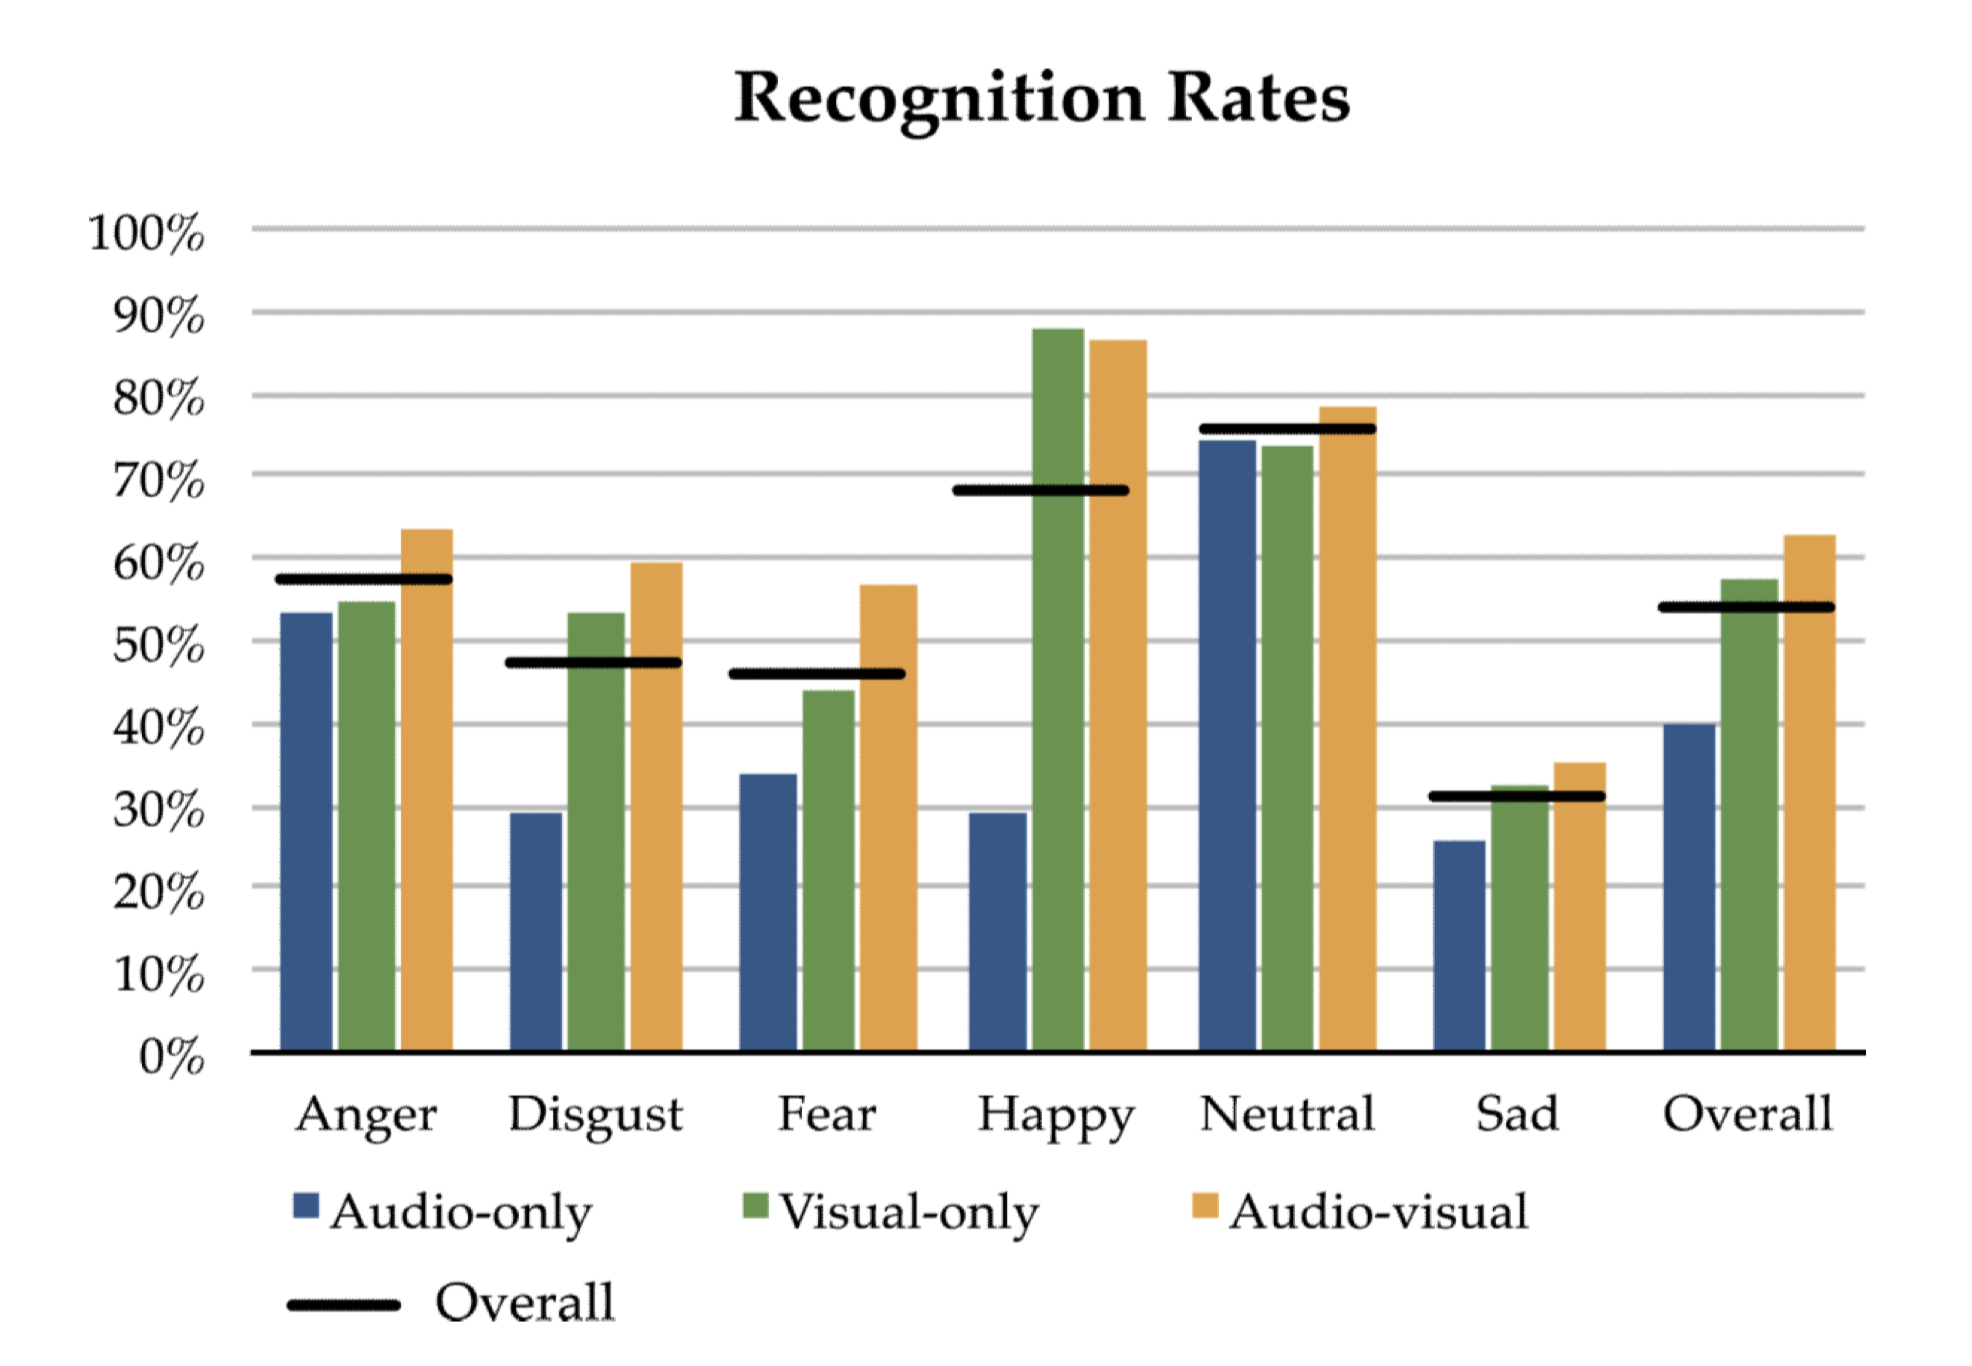
\includegraphics[width=0.8\textwidth]{res/crema.png}
    \caption{The results of the human annotation on the CREMA-D corpus \cite{cao2014crema}. There generally is a trend for audio-visual videos to be labelled better than visual-only data. There also seems to be a difference in accuracy depending on the emotion.}
    \label{fig:crema_results}
\end{figure}

Some questions remain unanswered. How do human annotators perform if they are confronted with still images of people talking? Are there any significant differences in accuracy depending on the phoneme that is spoken in the image? Those questions may help us in constructing a FER model that is robust against speech. 

Let us first analyse the performance of existing FER models against speaking subjects. Since our classic FER models are trained on single images, we will use still frames to evaluate them. With the help of the MFA (Section \ref{sub:mfa}) we were able to extract frames from the RAVDESS database (Section \ref{sub:ravdess}) with their respective phoneme labels. This allows us to analyse the phonetic bias of the model (Figure \ref{fig:phone_acc_ravdess}). The accuracy of our model differs depending on the phoneme. The best phonemes \texttt{Z} and \texttt{IY0} have accuracies of 49\%, whereas the worst performing phoneme \texttt{AY1} has an accuracy of only 40\%.

\begin{figure}
    \centering
    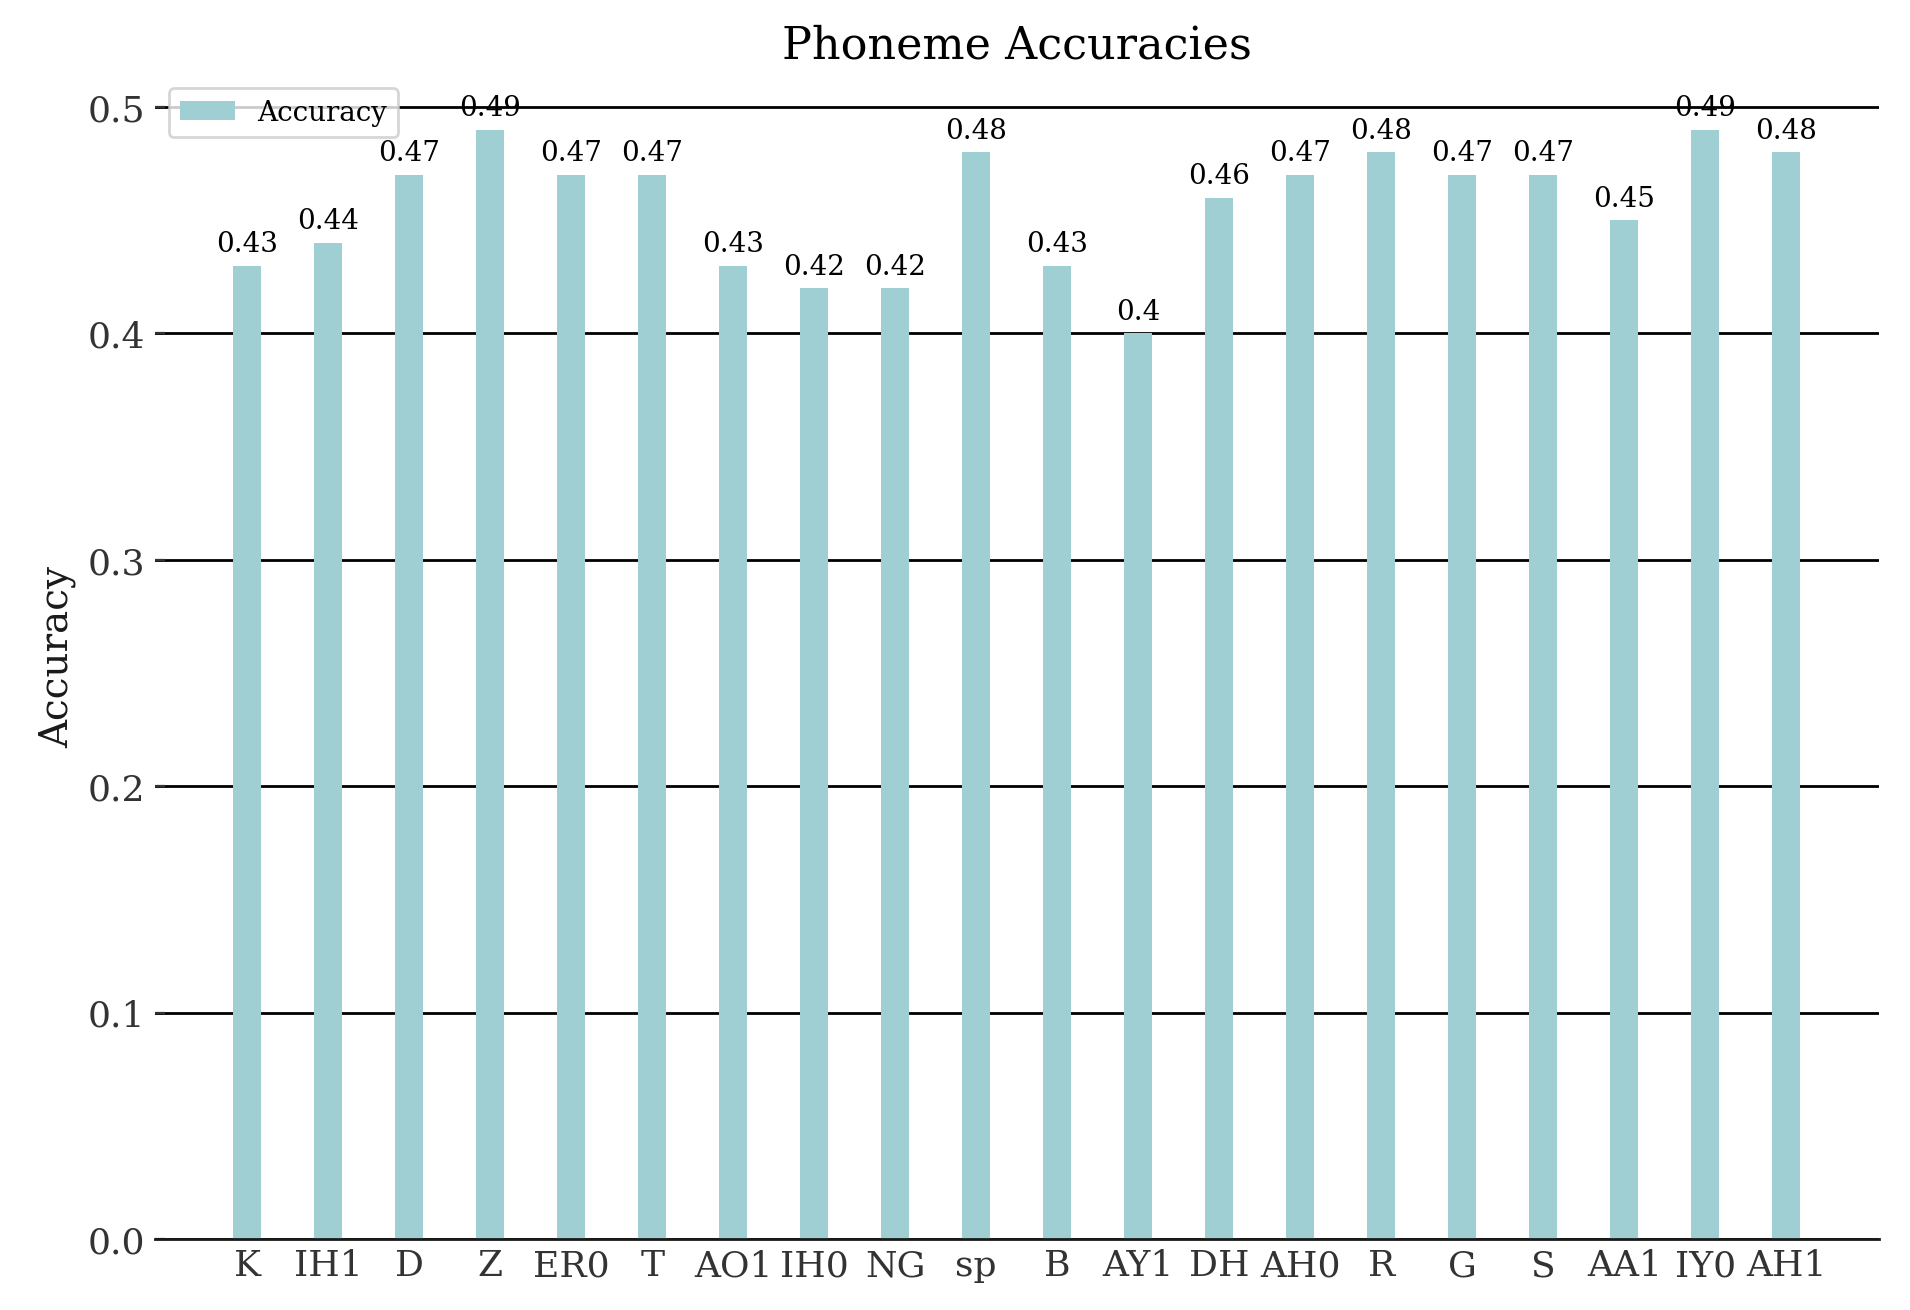
\includegraphics[width=0.8\textwidth]{res/phone_acc_model.png}
    \caption{Accuracies of our classic FER model depending on the phoneme that was spoken in the classified frame. Accuracies range from 40\% to 49\%, showing a significant bias on the spoken phonemes.}
    \label{fig:phone_acc_ravdess}
\end{figure}
\subsection{Goal}
We have seen that our classic FER models perform differently depending on the phoneme. Human annotators have differing performance based on emotions. An analysis on human bias depending on phoneme is however missing. Getting insights into human performance on emotion estimation depending on the spoken phoneme can help us in our task to build FER models that are more robust towards speech.

Is human bias similar to the bias shown in our models? Are humans capable to judge the emotional state of a speaking subject just by looking at a single frame, or does the performance increase when a video (without sound) is available? These are the questions we want to answer in this section.

\subsection{Setup and Material}
We turned to the RAVDESS dataset \cite{livingstone2018ryerson} for the material of our study. Compared to the CREMA-D corpus, RAVDESS also includes the \texttt{surprised} emotion, which will be part of our future models. We want our annotators to label the videos and selected still images from those videos. Given the size of the RAVDESS corpus, we decided to label a subset of the database. Videos of actors 4 (f), 5 (m), 9 (m), and 14 (f) were chosen, with two videos for each of the seven core emotions, ignoring \texttt{calm}. This amounts to $4 \cdot 7 \cdot 2 = 56$ videos. To keep the amount of image labels manageable for our annotators, we chose a subset of phonemes. Our choices were the phonemes \texttt{AY1}, \texttt{Z}, and \texttt{B}. They were chose due to their performance on the models, and occurrence in the videos. The total amount of images was 168, with each phoneme being represented 56 times.

To further split the workload between the annotators, the data was split into two groups. The first group was labelling videos and images from actors 4 and 5, and the second group was tasked with the data from actors 9 and 14. In total, each group had to label 28 videos and 84 images.

Annotators were first tasked with labelling the images before continuing to the videos. This was done to make sure that the labels for the images were not biased by the perception of the videos.

\subsection{Implementation}
The study was done through a simple web application. It was implemented using Svelte for the frontend application, while the data management and hosting was done through firebase. The annotations were saved in real-time, making sure that all completed labels were available in case of connection issues \cite{baur2021}.

\subsection{Annotators}
The annotators were recruited through personal contacts and a university seminar on a voluntary basis. In total, 16 participants annotated their batches. This leads to each data group being annotated eight times. All annotators were university students in their 20s.

Participants were prepared for the task through a presentation that was held in the seminar, or given in person. They were especially told not to take too much time on each datapoint, to make sure that their first impression was determining for the label.

\subsection{Results}
We will discuss the results of our study in more detail in section \ref{sec:discussion}. However some preliminary results are very interesting for our models and will be discussed here.

\paragraph{Temporal Dimension}
The annotators labelled both image and video data. The images are still frames from the videos. This allows us to compare the labelling performance between still frames and videos, and thus judge the importance of a temporal dimension. Our results, as seen in Figure \ref{fig:setting_overview}, conclude that 75.8\% of videos were labelled correctly, whereas the accuracy on the images was only 60.5\% (446 video labels, 1425 image labels). This leads us to believe that temporal data is very advantageous for FER purposes when the subject is talking.


\begin{figure}
    \centering
    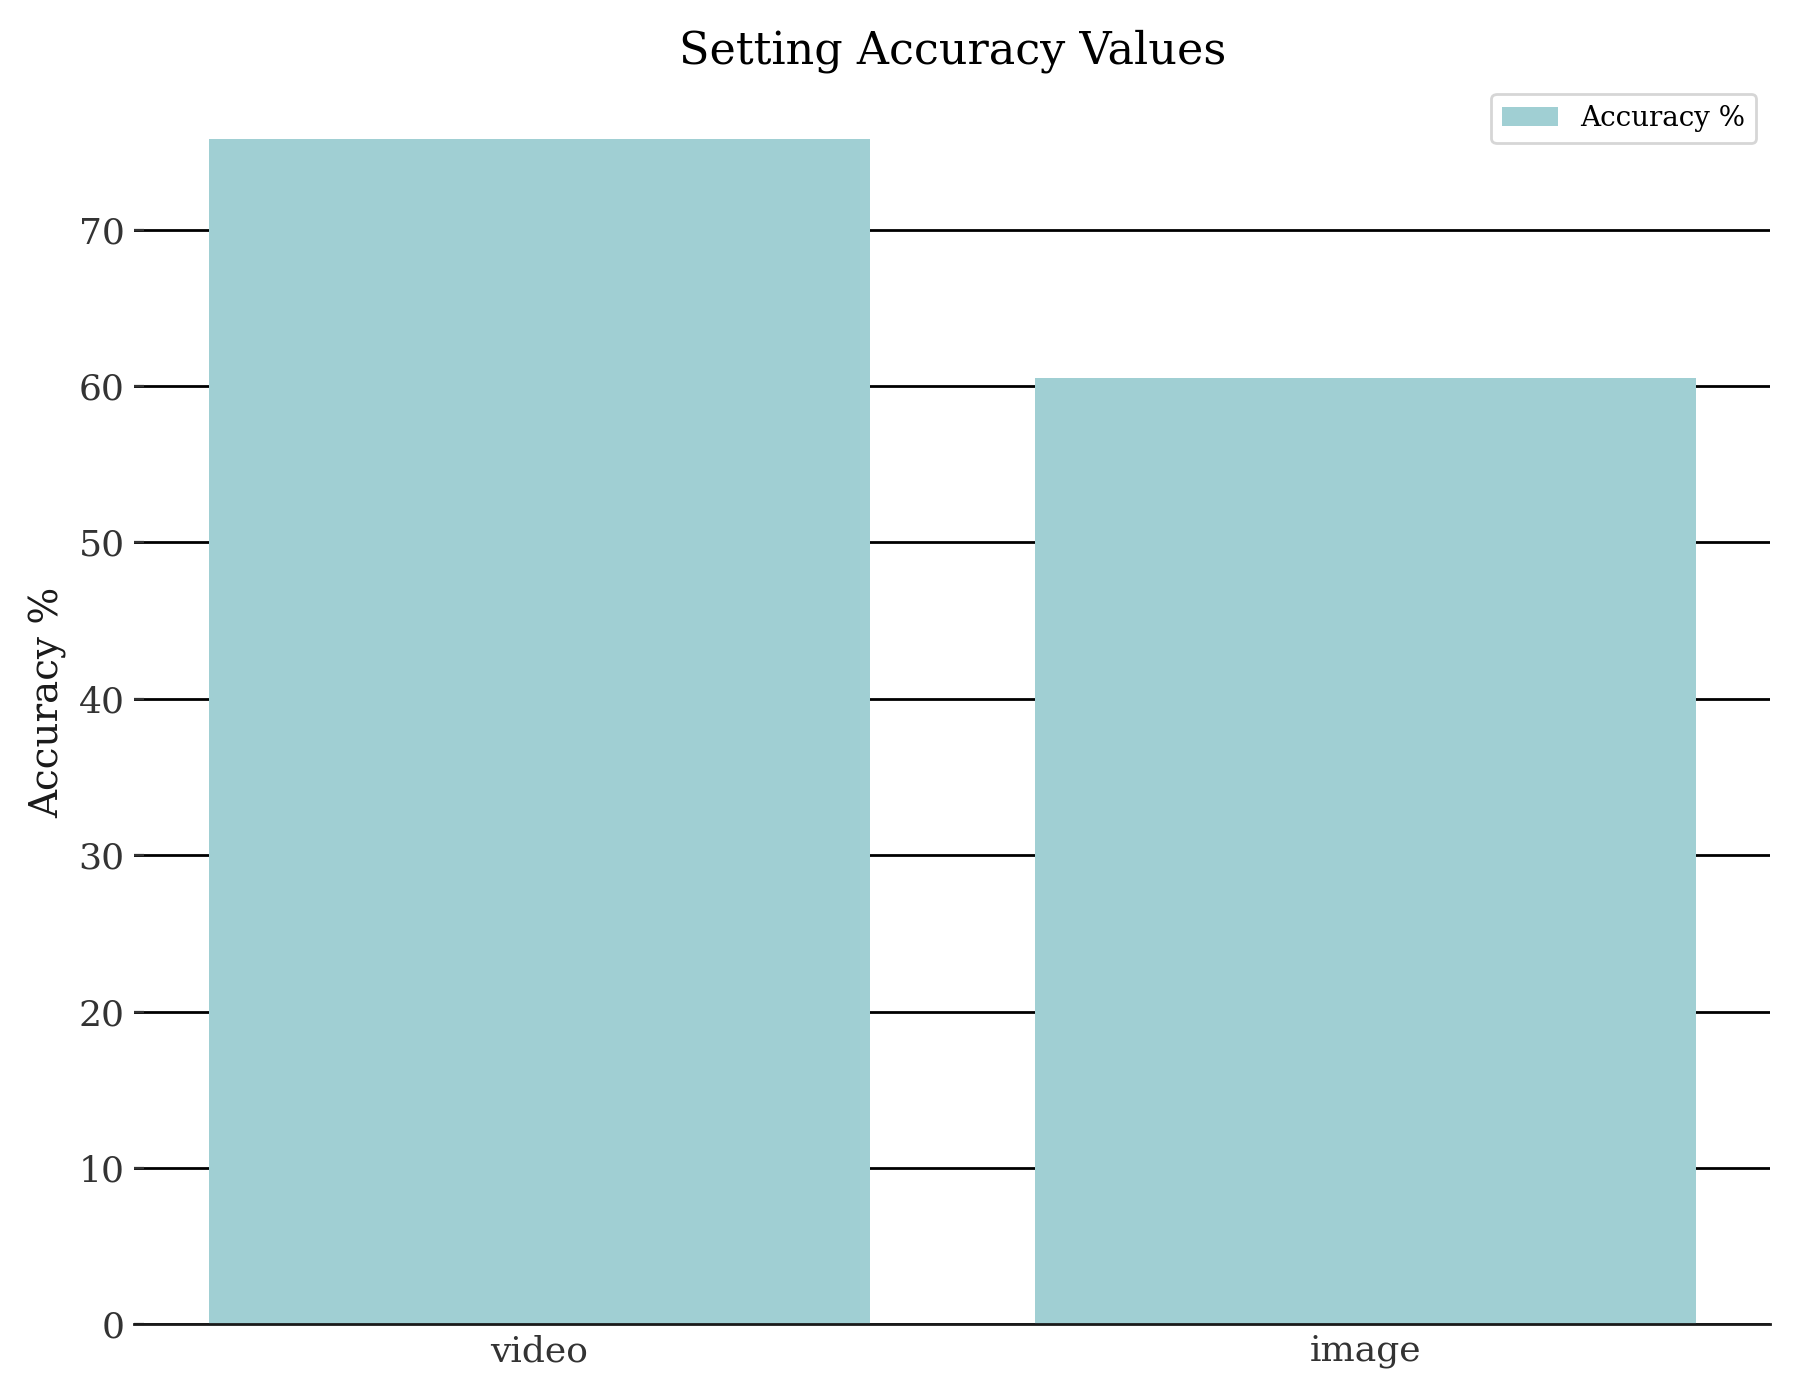
\includegraphics[width=0.65\textwidth]{res/Setting_overview.png}
    \caption{A comparison between the labelling accuracy of image and video data. The annotators did much better on video data, leading us to conclude that the temporal dimension is of high importance in FER during speech.}
    \label{fig:setting_overview}
\end{figure}

\paragraph{Lexical Compensation}
The labelled images were chosen on selected phonemes \texttt{AY1}, \texttt{Z}, and \texttt{B}. We can thus compare the annotator's accuracies on the individual phonemes. As seen before, there is a significant difference on the phonemes when our model labelled the images. The human annotators are consistently better, with an accuracy of 60\% across all phonemes. It seems like humans can compensate for the lexical content (the phonemes), which is something we want to include in our models.

\begin{figure}
    \centering
    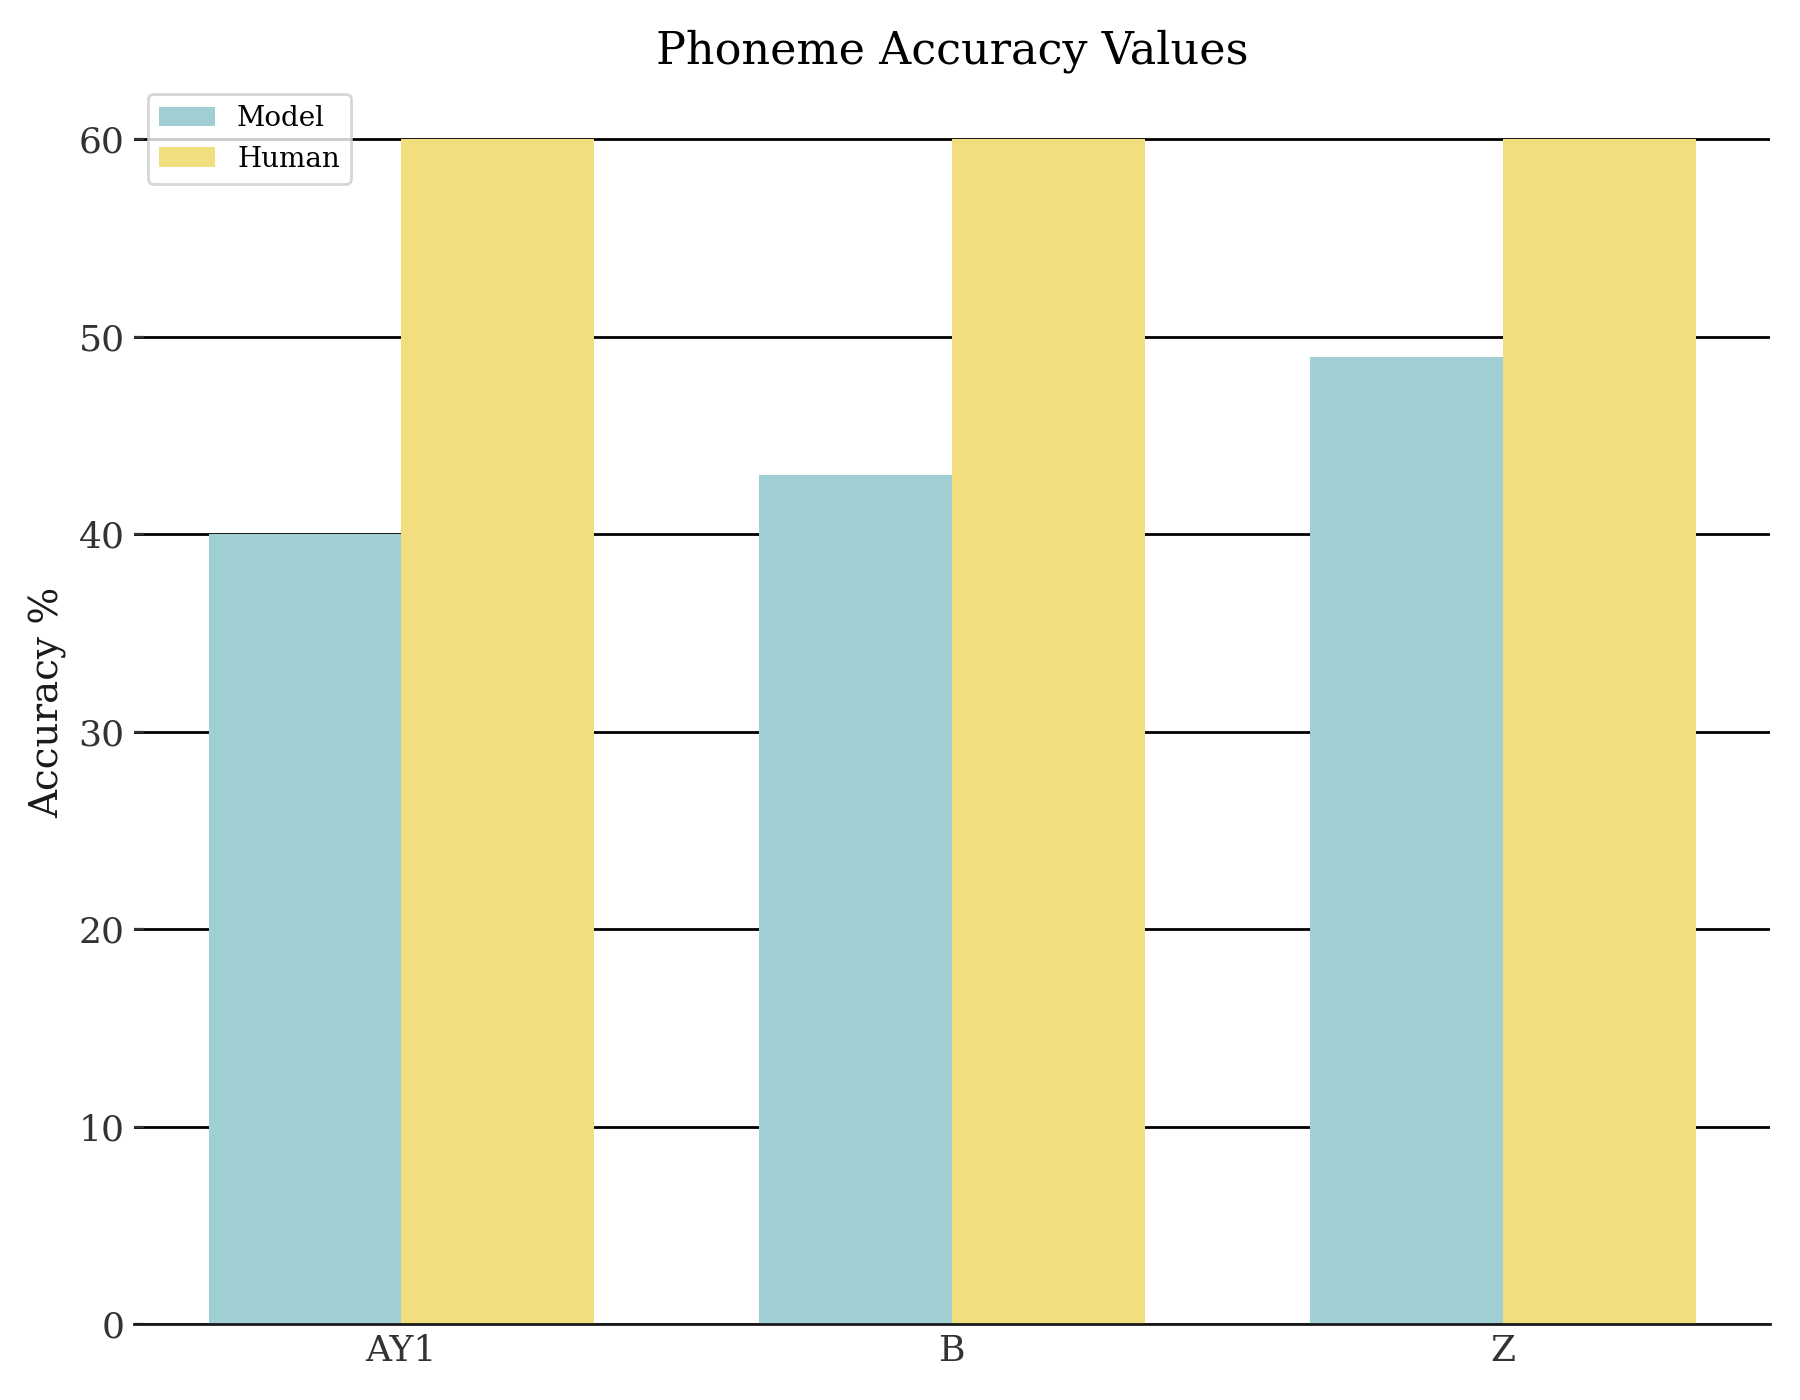
\includegraphics[width=0.65\textwidth]{res/Phone_model_acc.png}
    \caption{A comparison of the accuracies on the individual phonemes from the FER model and human annotators. The latter are better, while also having a consistent accuracy on the phonemes.}
    \label{fig:phone_model_human}
\end{figure}